\section{Umsetzung}
\label{sec:Umsetzung}

\subsection{Datengenerierung}
\label{sub:Datengenerierung}

Die zur Analyse genutzten Daten sind keine tatsächlichen Kundendaten, sondern wurden zum Zweck dieser Abschlussarbeit generiert.
Zur Generierung der Daten wurde ein Python Script benutzt. Das war notwendig, da in der aktuellen Version des IFP's die Widgetnamen nicht festgehalten werden. Dies war notwendig, da man in der aktuellen Implementierung nicht alle Widgets anhand der Logdateien erkennen kann. Selbst bei einer schnellen Auslieferung, wäre der Zeitraum zu klein, um genügend Kundendaten zu sammeln. Mithilfe eines Python und Bash Scripts wurden zufällig generierte Logfiles für einen Zeitraum von X generiert. 

\subsection{Grundlagen zum Elastic Stack}
\label{sub:Grundlagen zum Elastic Stack}
Um die Fragen aus der Problemstellung zu beantworten, wurde der Elastic Stack (ELK) benutzt. Der ELK besteht aus den Software Produkten Elasticsearch, Logstash und Kibana von der Firma Elastic N.V. Zusätzlich wurde noch Filebeat von der gleichen Firma benutzt. Die Funktionen der einzelnen Produkte werden in den nachfolgenden Unterkapiteln weiter erläutert. Die folgende Abbildung stellt den Workflow des Systems dar:

\begin{figure}[htb]
\begin{center}
	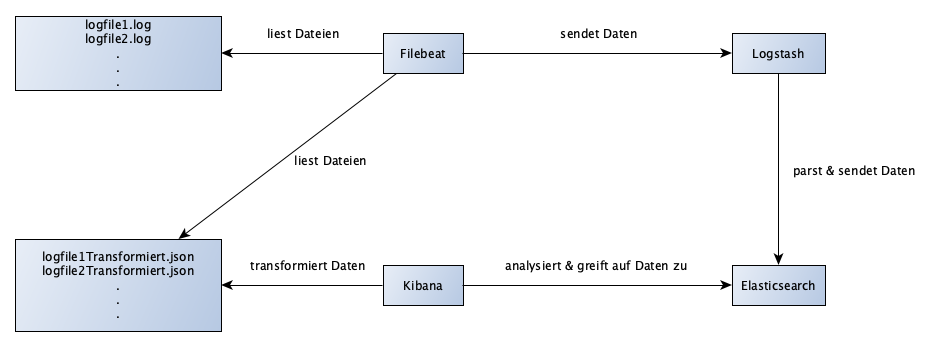
\includegraphics[width=430pt]{bilder/workflow.png}
\end{center}
\caption{ELK Workflow}
\label{fig:elk_workflow}
\end{figure}


\subsubsection{Filebeat}
\label{ssub:Filebeat}
Mit Filebeat können Dateien zeilenweise gelesen werden. In der Konfigurationsdatei von Filebeat gibt man an, wo und nach welchen Dateien gesucht werden soll. In unserem Fall waren es .log und .json Dateien. Außerdem kann man ein multiline pattern angeben, falls ein Eintrag mehrzeilig sein sollte. Die eingelesenen Dateien sendet Filebeat an Logstash weiter. Dabei merkt sich Filebeat welche Dateien schon gelesen wurden und welche Zeilen in diesen Dateien gelesen wurden. Das bedeutet ebenfalls, wenn eine komplett neue Datei oder eine neue Zeile in einer alten Datei auftaucht, merkt Filebeat das und liest es und sendet es wieder der an logstash. Damit ist die Echtzeitanalyse der Daten gewährleistet. 

\subsubsection{Logstash}
\label{sub:Logstash}
Die Aufgabe von Logstash ist es die Daten, von Filebeat zu empfangen und zu verarbeiten. Die empfangenen Daten befinden sich in einem rohen Zustand und werden mithilfe von mehreren Filter Plug-ins verarbeitet. Nachdem die Daten verarbeitet wurden sendet Logstash sie weiter an Elasticsearch.\\

\textbf{Grok Filter Plugin}\\
\\
Für die Logdateien wurde das Grok Filter Plug-in verwendet. In dem Grok-Filter gibt man einen regulären Ausdruck an, mitdem gematcht werden soll. Dabei kann man auch direkt festlegen, wie die Daten gespeichert werden sollen, falls gematcht wurde. Allgemein ist die Syntax dabei \%\{REGEXP:Feld\}. Neben einigen regulären Ausdrücken, die im Grok-Filter bereits implementiert sind (wie z.B. \textit{LOGLEVEL, TIMESTAMP\_ISO8601, SPACE, URIPATH}, uvm.) kann man auch eigene reguläre Ausdrücke definieren.
Wie schon in Kapitel \ref{ssub:Segmentierung} beschrieben, sollen die Daten segmentiert werden, was mit dem Grok-Filter realisiert werden kann. Z.B. kann man in dem regulären Ausdruck an der richtigen Stelle \textit{Incoming Request} setzen. Dadurch würden alle outgoing responses nicht matchen und auch nicht gespeichert werden. Außerdem kann man Daten matchen, aber keinem Feld zuweisen, wodurch sie auch nicht gespeichert werden. 
Die vollständige Konfiguration für die Logdateien sieht folgendermaßen aus:\\
\newpage
\begin{lstlisting}[caption = Sessionlog Filter,captionpos=b]
if [log][file][path] =~ "\S+session\S+" {
        grok{
            pattern_definitions => {
                "REQUEST" => "(Outgoing response|Incoming request)"
                "REQUEST_TYPE" => "(POST|GET)"
            }
            match => {"message" => [
                '^%{TIMESTAMP_ISO8601:zeit}%{SPACE}%{LOGLEVEL}%{SPACE}\[%{NOTSPACE:sessionid}\]\t\[%{NOTSPACE}\]\t\[%{NOTSPACE:userid}\]\t\[%{NOTSPACE} %{NOTSPACE}\]\t%{REQUEST:request}:%{SPACE}%{REQUEST_TYPE:request_type}%{SPACE}%{URIPATH:url}%{GREEDYDATA:stuff}',
                '^%{TIMESTAMP_ISO8601:zeit}%{GREEDYDATA:entry}'
                ]
            }
            remove_field => ['message']
        }

        if [url] !~ "\S+/rest" {
            drop{ }
        }

         mutate {
            gsub => [ "url", "\S+/rest", ""]
            remove_field => ['host','agent','@version','ecs','version']
        }

        date {
            match => [ "zeit", "ISO8601" ]
            target => "@timestamp"
		}

        if [request] == "Outgoing response"{
            drop { }
        }

        if [url] =~ "/fx/\S+" {
            mutate {
                gsub => ["url","/fx/\S+","/fx"]
            }
        }
\end{lstlisting}
\newpage
\label{lst:logEntryFilter}

\textbf{Ruby Filter Plugin}\\
\\
Das Ruby Filter Plugin wird benutzt, um transformierte Daten in Elasticsearch zu speichern. An dieser Stelle sei angemerkt, dass Elasticsearch zwar eine experimentelle \textit{transform} Funktion besitzt, diese aber für unseren Anwendungsfall (noch) nicht passend implementiert ist \citep{ElTr20}. Deshalb wurde ein Ruby Skript entwickelt, das diese Funktion ergänzt.\\

Die Daten, die nach dem Gedanken aus \ref{ssub:Feature_extraction} transformiert wurden, werden in einer JSON Datei gespeichert. Wie genau diese Daten aussehen bzw. wie sie zustande kommen wird in Kapitel \ref{ssub:Kibana} genaue erläutert. Zum besseren Verständis, wie das Ruby Skript arbeitet, wird an dieser Stelle daher die Datenstruktur abstrakt beschrieben.
Im Prinzip sind die Daten in 3 Ebenen aufgeteilt:\\
\begin{enumerate}
	\item UserIDs
	\item SessionIDs
	\item Widgets
\end{enumerate}
Dabei kann man die jeweils eine Ebene als ein Array verstehen. So besteht die oberste Ebene aus einem Array, das mit UserIDs gefüllt ist. Zu der UserID wird zusätzlich eine Array gespeichert, das aus SessionIDs besteht, die zu der UserID gehören. Zu diesen SessionIDs wird schließflich ebenfalls ein Array verknüpft, in dem festgehalten wird, welche Widgets in der Sesseion genutzt wurden und wie oft. Nun durchläuft das Skript also die beschriebenen Array Ebenen und speichert die gegebenen Daten in passende Felder, die schließlich an Elasticsearch gesendet und dort in einem passenden Index gespeichert werden.

\subsubsection{Elasticsearch}
\label{ssub:Elasticsearch}
Nachdem die von Filebeat gelesenen Daten von Logstash geparst wurden, werden die Daten in Elasticsearch gespeichert. Dabei werden die Logeinträge und die transformierten Daten seperat indiziert. Das bedeutet z.B., dass alle Einträge in den Logfiles vom 01.04.2020 und vom 02.04.2020 in eigenen Indizes gespeichert werden.

\subsubsection{Kibana}
\label{ssub:Kibana}
Kibana ist ein Tool, um die Daten, die in Elasticsearch gespeichert sind, zu visualisieren bzw. zu analysieren. Dabei liefert Kibana 
